27. \begin{figure}[ht!]
\center{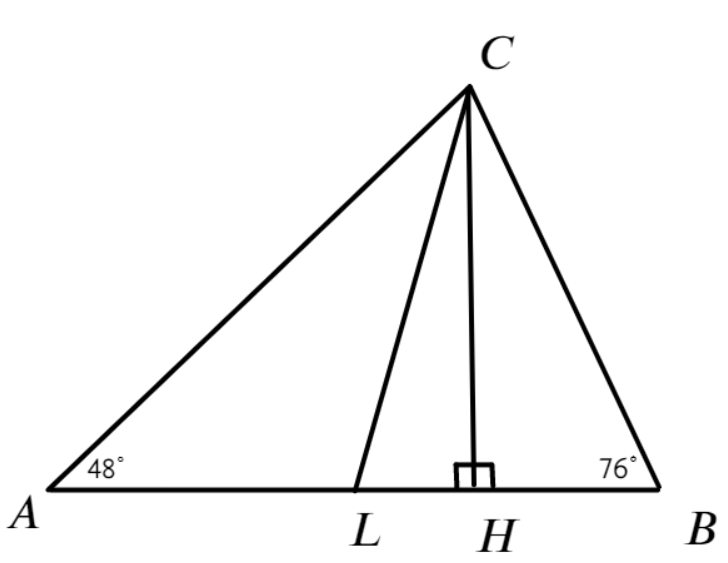
\includegraphics[scale=0.35]{g27.png}}
\end{figure}\\
$\angle C=180^\circ-\angle A-\angle B=180^\circ-48^\circ-76^\circ=56^\circ.$ Пусть $CH$ высота, а $CL$ --- биссектриса. Тогда $\angle BCH=90^\circ-76^\circ=14^\circ,$ а $\angle BCL=56^\circ:2=28^\circ.$ Таким образом, $\angle LCH=\angle BCL- \angle BCH=28^\circ-14^\circ=14^\circ.$\\
